\documentclass[12pt,a4paper]{report}

% Подгрузка пакетов для корректного и наиболее полного. должен грузиться как
% можно раньше, т.к. внутри себя определяет шрифты и некоторые прочие настройки,
% которые несколько не соответствуют тому, что надо.
\usepackage{amsmath,amsthm,amssymb}
\usepackage{cmap} %шобы пдф дружил с поиском и без диакритических знаков при копировании
% Позволяет использоваться текстовые кириллические индексы в формулах
\usepackage{mathtext}

% Отключаем масштабирование символов в многоэтажных дробях, индексах и пределах
% интегралов в соответствии с традицией русской типографской вёрстки
\everymath{\displaystyle}

% Увеличенные размеры символов в формулах
\DeclareMathSizes{12}{20}{14}{10}

% Подгрузка расширенной поддержки кириллицы
\usepackage[T1,T2A]{fontenc}

% Кодировка
\usepackage[utf8]{inputenc}

% Указываем, что пользоваться будем русским языком,
% подгружаем словари переносов, выставляются в соответствии с принятыми
% нормами отступы, интервалы между словами и пр.
\usepackage[russian]{babel}

% Поля по ГОСТ Р 7.0.11-2011
\usepackage[left=30mm, right=15mm, top=20mm, bottom=20mm]{geometry}

% Отступ первого абзаца главы
\usepackage{indentfirst}

% Выставлять полуторные интервалы в тексте, но не вмешивается в подписи, таблицы и сноски
\usepackage{setspace}

% Установка нужного шрифта
\renewcommand{\rmdefault}{ftm}

% Улучшенное форматирование таблиц
\usepackage{multirow,makecell,array}

% Красивые ссылки на литературу (конкретно, автоматическая сортировка и дефисы)
\usepackage{cite} 

% Отключаем перенос
\hyphenpenalty=10000 

% Работа с графикой
\usepackage{graphicx} 
\usepackage{float}

% Управление стилем оглавления
\usepackage{tocloft}  

% Устанавливаем шрифт 14 pt
\renewcommand{\tiny}{\fontsize{7}{8.4pt}\selectfont}
\renewcommand{\scriptsize}{\fontsize{9}{11pt}\selectfont}
\renewcommand{\footnotesize}{\fontsize{11}{13.6pt}\selectfont}
\renewcommand{\small}{\fontsize{12}{14.5pt}\selectfont}
\renewcommand{\normalsize}{\fontsize{14}{18pt}\selectfont}
\renewcommand{\large}{\fontsize{17}{20pt}\selectfont}
\renewcommand{\Large}{\fontsize{20}{25pt}\selectfont}

% Работа с библиографией
\makeatletter
% Оформляем библиографию в соответствии с ГОСТ 7.0.5
\bibliographystyle{utf8gost705u}
% Заменяем библиографию с квадратных скобок на точку	
%\renewcommand{\@biblabel}[1]{#1.}%
%\makeatother%

% Стили заголовков
\renewcommand{\thechapter}{\arabic{chapter}.} 
\renewcommand{\thesection}{\arabic{chapter}.\arabic{section}.}
\renewcommand{\thesubsection}{\arabic{chapter}.\arabic{section}.\arabic{subsection}.}
\renewcommand{\thefigure}{\thechapter\arabic{figure}}
\renewcommand{\thetable}{\thechapter\arabic{table}}

% По правилам нумеруются все заголовки вплоть до пунктов, так что выставляется 
% максимальная доступная по умолчанию глубина нумерации
\setcounter{secnumdepth}{5}   

% Позволяет сделать в полученной PDFке рабочими ссылки как в оглавлении, 
% так и в списке литературы и вообще в тексте
\usepackage{hyperref}
\providecommand{\phantomsection}{}

% Цвета
\usepackage{titlesec}
\usepackage[usenames]{color}
\usepackage{colortbl}

\begin{document}

% настройка отступов
\setlength{\parindent}{1.25cm} 
% убираем висячие строки  и подобное безобразие
\sloppy   
% Запрещаем разрыв страницы после первой строки абзаца
\clubpenalty=10000		
% Запрещаем разрыв страницы перед последней строкой абзаца
\widowpenalty=10000		

% Полуторный интервал
\onehalfspacing   

% Точки в оглавлении между названиями глав и номерами страниц
\renewcommand{\cftchapdotsep}{\cftdotsep} 

%%%%%%%%%%%%%%%%%%%%%%%%%%%%%%%%%%%%%%%%%%%%%%%%%%%%%%%%
%                    Титульный лист                    %
%%%%%%%%%%%%%%%%%%%%%%%%%%%%%%%%%%%%%%%%%%%%%%%%%%%%%%%%
\thispagestyle{empty}
\begin{titlepage}
\begin{center}
ФЕДЕРАЛЬНОЕ ГОСУДАРСТВЕННОЕ БЮДЖЕТНОЕ ОБРАЗОВАТЕЛЬНОЕ
УЧРЕЖДЕНИЕ ВЫСШЕГО ОБРАЗОВАНИЯ \\
«МОСКОВСКИЙ ГОСУДАРСТВЕННЫЙ УНИВЕРСИТЕТ\\
имени М.В.ЛОМОНОСОВА»
\vspace{1cm}

ФИЗИЧЕСКИЙ ФАКУЛЬТЕТ\\
\vspace{1cm}
КАФЕДРА ФИЗИКИ ПОЛУПРОВОДНИКОВ И КРИОЭЛЕКТРОНИКИ\\

\vspace{1cm}
БАКАЛАВРСКАЯ РАБОТА \\
\vspace{1cm}

\textbf{<<ИССЛЕДОВАНИЕ ТРАНСПОРТНЫХ ХАРАКТЕРИСТИК ОДНОЭЛЕКТРОННОГО ОДНОАТОМНОГО ТРАНЗИСТОРА>>}


\end{center}


\begin{flushright}
\vspace{1cm}

Выполнил студент \\
416 группы:\\

Назаров Степан Сергеевич \\

\underline{\hspace{3cm}}\\

\vspace{1cm}

Научный руководитель:\\
доцент, к.ф.\--м.н. Шорохов В.В. \\
\underline{\hspace{3cm}}\\
 
\end{flushright}

\vspace{1cm}
\begin{flushleft}
Допущена к защите \\
Зав. кафедрой профессор О.В.Снигирев

\underline{\hspace{3cm}} \\
\end{flushleft}
\begin{center}
\vspace{1cm}
\small МОСКВА \\ \number\year\normalsize
\end{center}
\end{titlepage}

%%%%%%%%%%%%%%%%%%%%%%%%%%%%%%%%%%%%%%%%%%%%%%%%%%%%%%%%
%                      Оглавление                      %
%%%%%%%%%%%%%%%%%%%%%%%%%%%%%%%%%%%%%%%%%%%%%%%%%%%%%%%%
\tableofcontents

% Стили заголовков:
% \chapter{Название} для названий глав
% \section{Название} для заголовков второго уровня
% \subsection{Название} для заголовков третьего уровня

% Для заголовков без нумерации 
% \chapter*{Название}  % Сам заголовок
% \addcontentsline{toc}{chapter}{Название}  % Добавление в оглавление

\titleformat{\chapter}
    {\phantomsection \filright}
    {\thechapter}
    {1em}
    {}

\titleformat{name=\chapter,numberless}[block]
    {\phantomsection \filcenter}
    {}
    {1em}
    {\newcommand{\thischaptername}}
    [\MakeUppercase{\thischaptername}\addcontentsline{toc}{chapter}{\thischaptername}]

\titleformat{\section}
    {\phantomsection \filright}
    {\thesection}
    {1em}
    {}

\titleformat{\subsection}
    {\phantomsection \filright}
    {\thesubsection}
    {1em}
    {}


%%%%%%%%%%%%%%%%%%%%%%%%%%%%%%%%%%%%%%%%%%%%%%%%%%%%%%%%
%                     Текст работы                     %
%%%%%%%%%%%%%%%%%%%%%%%%%%%%%%%%%%%%%%%%%%%%%%%%%%%%%%%%


\chapter*{Введение}

%Работа первого одноэлектронного транзистора была продемонстрирована ещё в 1987 г.  \cite{Fulton_Dolan}. Основным принципом работы данного устройства является коррелированный во времени и пространстве транспорт электронов. Для 

Одноэлектронные устройства — это такие устройства, принцип работы которых основан на явлении коррелированного в пространстве и времени транспорта единичных электронов. Обязательным требованием к таким устройствам является достаточно высокое значение собственных и взаимных ёмкостей электродов и зарядовых островков. Это необходимо для того, чтобы изменение электростатической энергии системы за единичный акт туннелирования электрона было много больше энергии тепловых флуктуаций.

Первые работы, сообщающие о реализации устройств данного типа появились более 30 лет назад \cite{Fulton_Dolan, Amman, Likharev} и нашли применения в самых разных сферах: сенсоры\cite{sensor}, термометрия\cite{Thermo}, память\cite{memory}.

Развитие технологических процессов в области изготовления полупроводниковых изделий и материалов, привело к увеличению разрешающей способности, что позволяет уменьшить характерные размеры островков в устройствах. В наши дни на передовой находятся устройства с одиночными молекулами или атомами в роли зарядового центра \cite{SASET_EXP_OUR, SMSET}. Уменьшение размеров островков ведёт к возможности работы устройств при более высоких температурах (вплоть до комнатной? ссылка??????). 

Пока не существует технологического процесса, позволяющего в производственных масштабах изготавливать структуры из единичных атомов с допусками в единицы ангстрем. Однако, с точки зрения практических применений (создание сенсоров, логических элементов) проявляется к элементам из одиночных атомов и молекул, а в перспективе к элементам с атомной функциональной структурой. А значит, существование универсальных методик расчёта для таких структур необходимо для проектирования устройств с реальными практическими применениями.

тут ещё желательно что-нибудь написать и отредактировать то, что выше

\section*{Цель работы}

Целью данной бакалаврской работы является создание универсального алгоритма расчёта структур с атомной функциональной структурой, анализ и моделирование систем с такими структурами в роли ключевых элементов и применение данного алгоритма для объяснения наблюдаемых в эксперименте характеристик одноатомных одноэлектронных устройств.

\chapter{Двухуровневая система}

Одноэлектронный транзистор состоит из маленького металлического островка субмикронных размеров, двух электродов исток-сток соединённых с островком туннельно и электрода затвор, изолированного от острова. Схематично это устройство изображено на рис. \ref{fig:SET}. На рисунке так же указаны параметры: $C_S, C_D, C_G$ — ёмкости соответствующих переходов; $R_S, R_D$ — соответствующие туннельные сопротивления.

\begin{figure}
	\center{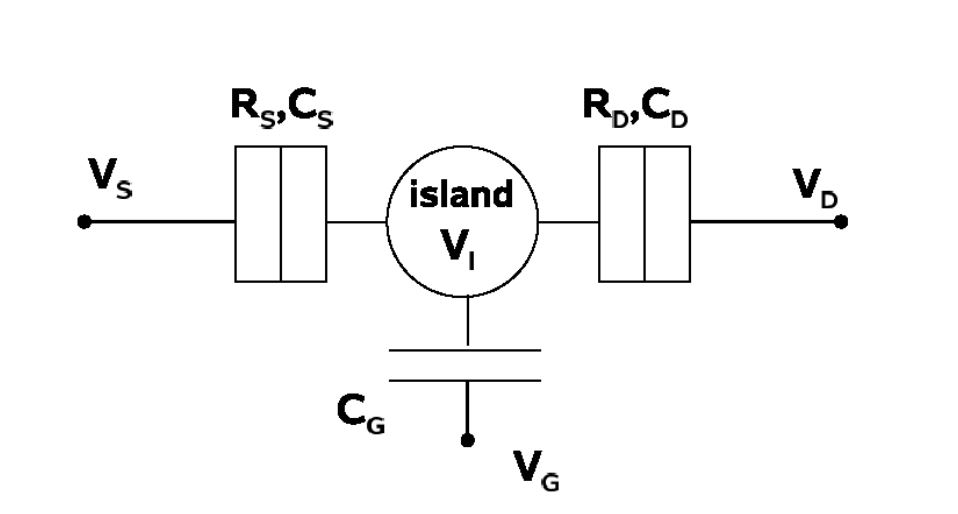
\includegraphics[scale=0.3]{SET.jpg}}
	\caption{Одноэлектронный транзистор}
	\label{fig:SET}
\end{figure}

Работа такого транзистора возможна только при выполнении двух очень важных условий:
\begin{equation}\label{c1}
\frac{e^2}{2C} >> kT
\end{equation}
\begin{equation}\label{c2}
R_S >> R_Q, R_D >> R_Q,  R_Q = h/e^2
\end{equation}
\section{kek}
\begin{equation}\label{c3}
R_S >> R_Q, R_D >> R_Q,  R_Q = h/e^2
\end{equation}
Velit aliqua irure do adipisicing enim sunt proident laboris enim. Mollit laborum ex excepteur incididunt laboris labore quis velit ut. Dolore anim nostrud officia cupidatat anim. Elit dolore quis consequat laboris sunt ad commodo. Consequat deserunt tempor non nulla sit ipsum irure labore ipsum duis elit commodo magna est. Consectetur non ad excepteur nostrud exercitation dolore cillum mollit proident occaecat aliqua enim exercitation. Esse deserunt occaecat est aliqua.

Occaecat reprehenderit deserunt culpa ea eiusmod. Fugiat voluptate veniam officia velit culpa Lorem consequat nostrud cupidatat magna duis sunt nisi occaecat. In sint occaecat aliqua ad qui esse deserunt ad veniam ex eu. Elit amet tempor anim magna occaecat incididunt ut. Aute sunt dolor proident et cupidatat eu et et irure proident. Do magna eiusmod reprehenderit dolore esse elit amet laborum ea veniam adipisicing commodo pariatur esse.

Commodo nisi quis est sint cupidatat. Mollit sint nostrud labore ipsum enim non nulla veniam voluptate est cillum sunt eiusmod deserunt. Incididunt eu exercitation elit consequat officia do non ut. Ullamco cillum officia minim consectetur reprehenderit deserunt in.

Magna magna eiusmod nulla sint nostrud tempor minim eu laborum. Ullamco irure eiusmod pariatur velit laboris. Culpa tempor ea voluptate reprehenderit ex velit in amet irure adipisicing mollit. Quis excepteur non sit labore aute. Veniam ex incididunt excepteur adipisicing.

Tempor cillum velit ullamco eiusmod consectetur et do. Velit adipisicing do mollit enim voluptate fugiat excepteur elit veniam magna culpa adipisicing sit. Lorem magna sit veniam cupidatat et esse ex id.



\chapter*{Выводы}

Non adipisicing sint ut incididunt duis ut duis cillum sit pariatur tempor enim commodo officia. Non nostrud laborum esse dolor est veniam. Et sunt et tempor aute reprehenderit ea ex Lorem officia. Aute magna nisi ullamco proident id aliqua ex eiusmod eu commodo ullamco. Officia veniam in consectetur deserunt ex laborum pariatur proident sunt. Nostrud deserunt eiusmod aliqua cupidatat eiusmod adipisicing officia aute. Duis aute enim ex ullamco in cupidatat aute irure mollit occaecat sint irure. Cupidatat occaecat id excepteur duis eu quis nisi incididunt. Deserunt aliqua pariatur do nostrud nisi qui reprehenderit reprehenderit cillum deserunt proident ipsum.


\chapter*{Заключение}

Esse ex eiusmod id velit eu occaecat nisi occaecat dolor id anim esse. Quis sunt elit consequat excepteur ut ex sit dolore ad. Est irure tempor pariatur magna voluptate pariatur est. Commodo commodo fugiat sunt non. Laboris occaecat voluptate Lorem consequat aute consectetur non sunt mollit fugiat eiusmod aute adipisicing. Laboris officia nisi officia id ea consectetur laborum cillum aliquip ad laborum reprehenderit. Dolor veniam nulla ad pariatur nisi mollit consectetur sint. Nostrud ipsum dolor sunt amet veniam fugiat. Et labore anim sint nostrud. Non adipisicing sint aute duis irure commodo esse. Ea exercitation elit fugiat dolor. Nostrud eu fugiat cupidatat aliquip veniam deserunt nulla sint culpa et irure.

%%%%%%%%%%%%%%%%%%%%%%%%%%%%%%%%%%%%%%%%%%%%%%%%%%%%%%%%
%                     Библиография                     %
%%%%%%%%%%%%%%%%%%%%%%%%%%%%%%%%%%%%%%%%%%%%%%%%%%%%%%%%
% Меняем заголовок у библиографии
\renewcommand\bibname{Cписок литературы}

\begin{thebibliography}{99}
    % Пример оформления источника
    % \bibitem{Sabbas} São Sabbas F. et al. Statistical analysis of space–time relationships between sprites and lightning // Journal of Atmospheric and Solar-Terrestrial Physics. 2003. vol. 65, number 5. p. 525-535.
	\bibitem{Fulton_Dolan} T. A. Fulton and G. J. Dolan. Phys. Rev. Lett., 59:109–112, Jul 1987.
	\bibitem{Amman}M. Amman, K. Mullen, and E. Ben-Jacob. Journal of Applied Physics, 65(1):339–346,
1989.
	\bibitem{Likharev}D.V. Averin and K.K. Likharev. Single electronics: A correlated transfer of single
electrons and cooper pairs in systems of small tunnel junctions. In B.L. ALTSHULER,
P.A. LEE, and R.A. WEBB, editors, Mesoscopic Phenomena in Solids, volume 30 of
Modern Problems in Condensed Matter Sciences, chapter 6, pages 173–271. Elsevier,
1991.
	\bibitem{Landau}Л.Д.Ландау, Е.М.Лифшиц Электродинамика сплошных сред М., Наука, 1982
	\bibitem{Thermo} J. P. Pekola, J. K. Suoknuuti, J. P. Kauppinen, M. Weiss, P. v. d. Linden, and A. G. M.
Jansen. Coulomb blockade thermometry in the milli-kelvin temperature range in high
magnetic fields. Journal of Low Temperature Physics, 128(5):263–269, Sep 2002.
	\bibitem{memory} K. Nakazato, R. J. Blaikie, and H. Ahmed. Single-electron memory. Journal of Applied
Physics, 75(10):5123–5134, 1994.
	\bibitem{sensor} Knobel, R., Cleland, A. Nanometre-scale displacement sensing using a single electron transistor. Nature 424, 291–293 (2003).
	\bibitem{SASET_EXP_OUR} V. V. Shorokhov, D. E. Presnov, S. V. Amitonov, Yu. A. Pashkin, and V. A. Krupenin.Single-electron tunneling through an individual arsenic dopant in silicon
Nanoscale, 9:613–620, 2017.
	\bibitem{SMSET} Kubatkin, S., Danilov, A., Hjort, M. et al. Single-electron transistor of a single organic molecule with access to several redox states. Nature 425, 698–701 (2003).
\end{thebibliography}
\end{document}
